In principle, our approach applies to linear dynamics and measurement models $\mathbf{f}$ and $\mathbf{h}$. However, since the robot will be controlled stay close to the nominal plan during execution, we can approximate the nonlinear dynamics and measurement models with local linearizations around the plan. The linear(ized) models can be expressed in terms of deviation from the true state $\bar{\mathbf{x}}_t = (\mathbf{x}_t - \mathbf{x}^{\star}_{t})$, control input deviation $\bar{\mathbf{u}}_t = (\mathbf{u}_t - \mathbf{u}^{\star}_{t})$, and deviation from the actual measurement $\bar{\mathbf{z}}_t = (\mathbf{z}_t - \mathbf{h}[\mathbf{x}^{\star}_{t}, \mathbf{0}])$, as:
\begin{align}
\bar{\mathbf{x}}_t &= A_t\bar{\mathbf{x}}_{t-1} + B_t\bar{\mathbf{u}}_{t-1} + V_t\mathbf{m}_t, ~~ \mathbf{m}_t \sim \mathcal{N} [\mathbf{0}, M_t] \label{eq:lindynmodel} \\
\bar{\mathbf{z}}_t &= H_t\bar{\mathbf{x}}_{t} + W_t\mathbf{n}_t, ~~~~~~~~~~~~~~~~ \mathbf{n}_t \sim \mathcal{N} [\mathbf{0}, N_t]. \label{eq:linobsmodel}
\end{align}
where the Jacobians matrices of $\mathbf{f}$ and $\mathbf{h}$ are given by:
\begin{align} \label{eq:jacobians}
& ~~~~~ A_t = \frac{\partial\mathbf{f}}{\partial\mathbf{x}}[\mathbf{x}^{\star}_{t-1}, \mathbf{u}^{\star}_{t-1},\mathbf{0}], ~ B_t = \frac{\partial\mathbf{f}}{\partial\mathbf{u}}[\mathbf{x}^{\star}_{t-1}, \mathbf{u}^{\star}_{t-1},\mathbf{0}],\\
& V_t = \frac{\partial\mathbf{f}}{\partial\mathbf{m}}[\mathbf{x}^{\star}_{t-1}, \mathbf{u}^{\star}_{t-1},\mathbf{0}],~ H_t = \frac{\partial\mathbf{h}}{\partial\mathbf{x}}[\mathbf{x}^{\star}_{t}, \mathbf{0}],~ W_t = \frac{\partial\mathbf{h}}{\partial\mathbf{n}}[\mathbf{x}^{\star}_{t}, \mathbf{0}] \nonumber.
\end{align}

The true state $\mathbf{x}_t$, and hence the true state deviation $\bar{\mathbf{x}}_t$, is not available during actual execution. We use a Kalman filter to keep track of an estimate of the state deviation $\hat{\mathbf{x}}_t = \mathrm{E}[\bar{\mathbf{x}}_t]$. The estimate of the state deviation evolves according to:
\vspace*{-3pt}
\begin{equation} \label{eq:Kalman}
\hat{\mathbf{x}}_t = K_t\bar{\mathbf{z}}_t + (I - K_tH_t)(A_t \hat{\mathbf{x}}_{t-1} + B_t \bar{\mathbf{u}}_{t-1}),
\end{equation}
where $K_t$ is the Kalman gain matrix \cite{Book:Simon06}. To compensate for the uncertainty, the robot is controlled using a linear feedback policy related to the estimate of the state deviation as:
\vspace*{-3pt}
\begin{equation} \label{eq:controlpolicy}
\bar{\mathbf{u}}_t = L_{t+1}\hat{\mathbf{x}}_{t},
\end{equation}
where $L_t$ is the control gain matrix determined by the choice of feedback controller \cite{Book:Stengel94}.

\subsection{A Priori State Distributions}

Under the given assumptions, the probability distributions of the robot state can be characterized a priori i.e., before execution. Combining Eqns. (\ref{eq:lindynmodel}), (\ref{eq:linobsmodel}), (\ref{eq:Kalman}), and (\ref{eq:controlpolicy}), the true state deviation $\bar{\mathbf{x}}_t$, and the estimate $\hat{\mathbf{x}}_t$, jointly evolve as \cite{vandenBerg11_IJRR}:
\begin{align}\label{eq:jointevolve}
\begin{bmatrix} \bar{\mathbf{x}}_t \\ \hat{\mathbf{x}}_t \end{bmatrix} =& \begin{bmatrix} A_t & B_tL_t \\ K_tH_tA_t & A_t + B_tL_t - K_tH_tA_t \end{bmatrix} \begin{bmatrix} \bar{\mathbf{x}}_{t-1} \\ \hat{\mathbf{x}}_{t-1} \end{bmatrix} + \\ & \begin{bmatrix} V_t & 0 \\ K_tH_tV_t & K_tW_t \end{bmatrix} \begin{bmatrix} \mathbf{m}_t \\ \mathbf{n}_t \end{bmatrix}, ~ \begin{bmatrix} \mathbf{m}_t \\ \mathbf{n}_t \end{bmatrix} \sim \mathcal{N}[\mathbf{0}, \begin{bmatrix} M_t & 0 \\ 0 & N_t \end{bmatrix}] \nonumber.
\end{align}
We can write this equation in shorthand (for appropriate definitions of $\mathbf{y}_t$, $\mathbf{q}_t$, $F_t$, $G_t$, and $Q_t$) as:
\begin{equation}
\mathbf{y}_t = F_t\mathbf{y}_{t-1} + G_t\mathbf{q}_{t}, ~ \mathbf{q}_t \sim \mathcal{N}[\mathbf{0}, Q_t].
\end{equation}
The mean $\hat{\mathbf{y}}_t \in \mathbb{R}^{2n_x}$ and associated variance $R_t = \mathrm{Var}[\mathbf{y}_t]$, propagate according to:
\begin{align}
\hat{\mathbf{y}}_t &= F_t\hat{\mathbf{y}}_{t-1}, ~~~~~~~~~~~~~~~~~~~ \hat{\mathbf{y}}_0 = \mathbf{0}, \label{eq:oldjointmean}\\
R_t &= F_tR_{t-1}F_t^T + G_tQ_tG_t^T, ~~ R_0 = \begin{bmatrix} \mathrm{Var}[\bar{\mathbf{x}}_0] & 0 \\ 0 & 0 \end{bmatrix}. \label{eq:oldjointvar}
\end{align}
The \emph{unconditional} a priori distribution of the state $\mathbf{x}_t$ at stage $t$ is given by the marginal $\mathbf{x}_t \sim \mathcal{N}[(\mathbf{x}^{\star}_t + \Lambda \hat{\mathbf{y}}_t), \Lambda R_t \Lambda^T]$, where $\Lambda = \left[ I ~~ 0  \right]$. %The unconditional distribution assumes that the probabilities of collision are independent at each stage of the plan.

To accurately estimate the probability of collision, we need to estimate the a priori state distributions at each stage along the plan that are \emph{conditioned} on the previous stages being collision free, i.e. the distribution $(\mathbf{x}_t\;|\;\bigwedge_{i=0}^{t-1} \mathbf{x}_i \in \mathcal{X}_F)$. To this end, we pursue a recursive approach similar as above to propagate the conditional distributions.

Let $\mathbf{y}_{t|s}$ denote the joint distribution of the true state deviation and its estimate at time $t$ conditioned on the state being collision free for all stages $0,\ldots,s$:
\begin{align}
\mathbf{y}_{t|s} = (\begin{bmatrix} \bar{\mathbf{x}}_t \\ \hat{\mathbf{x}}_t \end{bmatrix} \; | \; \bigwedge_{i=0}^s \; \mathbf{x}_i \in \mathcal{X}_F).
\end{align}
We then repeatedly, for each stage $t$ of the plan, carry out the following steps. Assume we are given the joint conditional distribution $\mathbf{y}_{t|t-1}$ as approximated by a Gaussian distribution $\mathcal{N}[\hat{\mathbf{y}}_{t|t-1}, R_{t|t-1}]$. We then approximate the distribution $\mathbf{y}_{t|t}  \sim \mathcal{N}[\hat{\mathbf{y}}_{t|t}, R_{t|t}]$ of all collision-free states at stage $t$ by truncating the distribution $\mathbf{y}_{t|t-1}$ against the obstacles in the environment. Truncating the distribution effectively discounts all colliding states from the distribution (Fig. \ref{fig:teaser}), and results in a shift of the mean and variance by $\Delta \mathbf{y}_t$ and $\Delta R_{t-1}$ (as detailed in Sec.\ \ref{sec:trunc}), respectively:
\begin{align}
\hat{\mathbf{y}}_{t|t} & = \hat{\mathbf{y}}_{t|t-1} - \Delta \mathbf{y}_t \\
R_{t|t} & = R_{t|t-1} - \Delta R_t
\end{align}
Using Eqns. (\ref{eq:oldjointmean}) and (\ref{eq:oldjointvar}), the conditional mean and variance are then propagated according to:
\begin{align}
\hat{\mathbf{y}}_{t+1|t} &= F_{t+1} \hat{\mathbf{y}}_{t|t}, \label{eq:newjointmean}\\
R_{t+1|t} &= F_{t+1}R_{t|t}F_{t+1}^T + G_{t+1}Q_{t+1}G_{t+1}^T. \label{eq:newjointvar}
\end{align}
The recursion then continues. The initial conditions are set by defining $\hat{\mathbf{y}}_{0|-1} = \hat{\mathbf{y}}_0 = \mathbf{0}$ and $R_{0|-1} = R_0 = \left[\begin{smallmatrix} \mathrm{Var}[\bar{\mathbf{x}}_0] & 0 \\ 0 & 0 \end{smallmatrix} \right]$.

At each stage of the recursion, the marginal $\mathbf{x}_{t|t-1} \sim \mathcal{N}[(\mathbf{x}^{\star}_t + \Lambda \hat{\mathbf{y}}_{t|t-1}), \Lambda R_{t|t-1} \Lambda^T]$ of the joint distribution $\mathbf{y}_{t|t-1}$ gives the a priori distribution of the robot state $\mathbf{x}_t$, given that all the previous states $[\mathbf{x}_0,\ldots,\mathbf{x}_{t-1}]$ are collision free. When this distribution is truncated against the obstacles, an accurate estimate is obtained of the conditional probability of collision at stage $t$ (as detailed in Sec.\ \ref{sec:estprob}).

\subsection{Truncating A Priori Distributions} \label{sec:trunc}

\begin{figure*}[t]
\centering
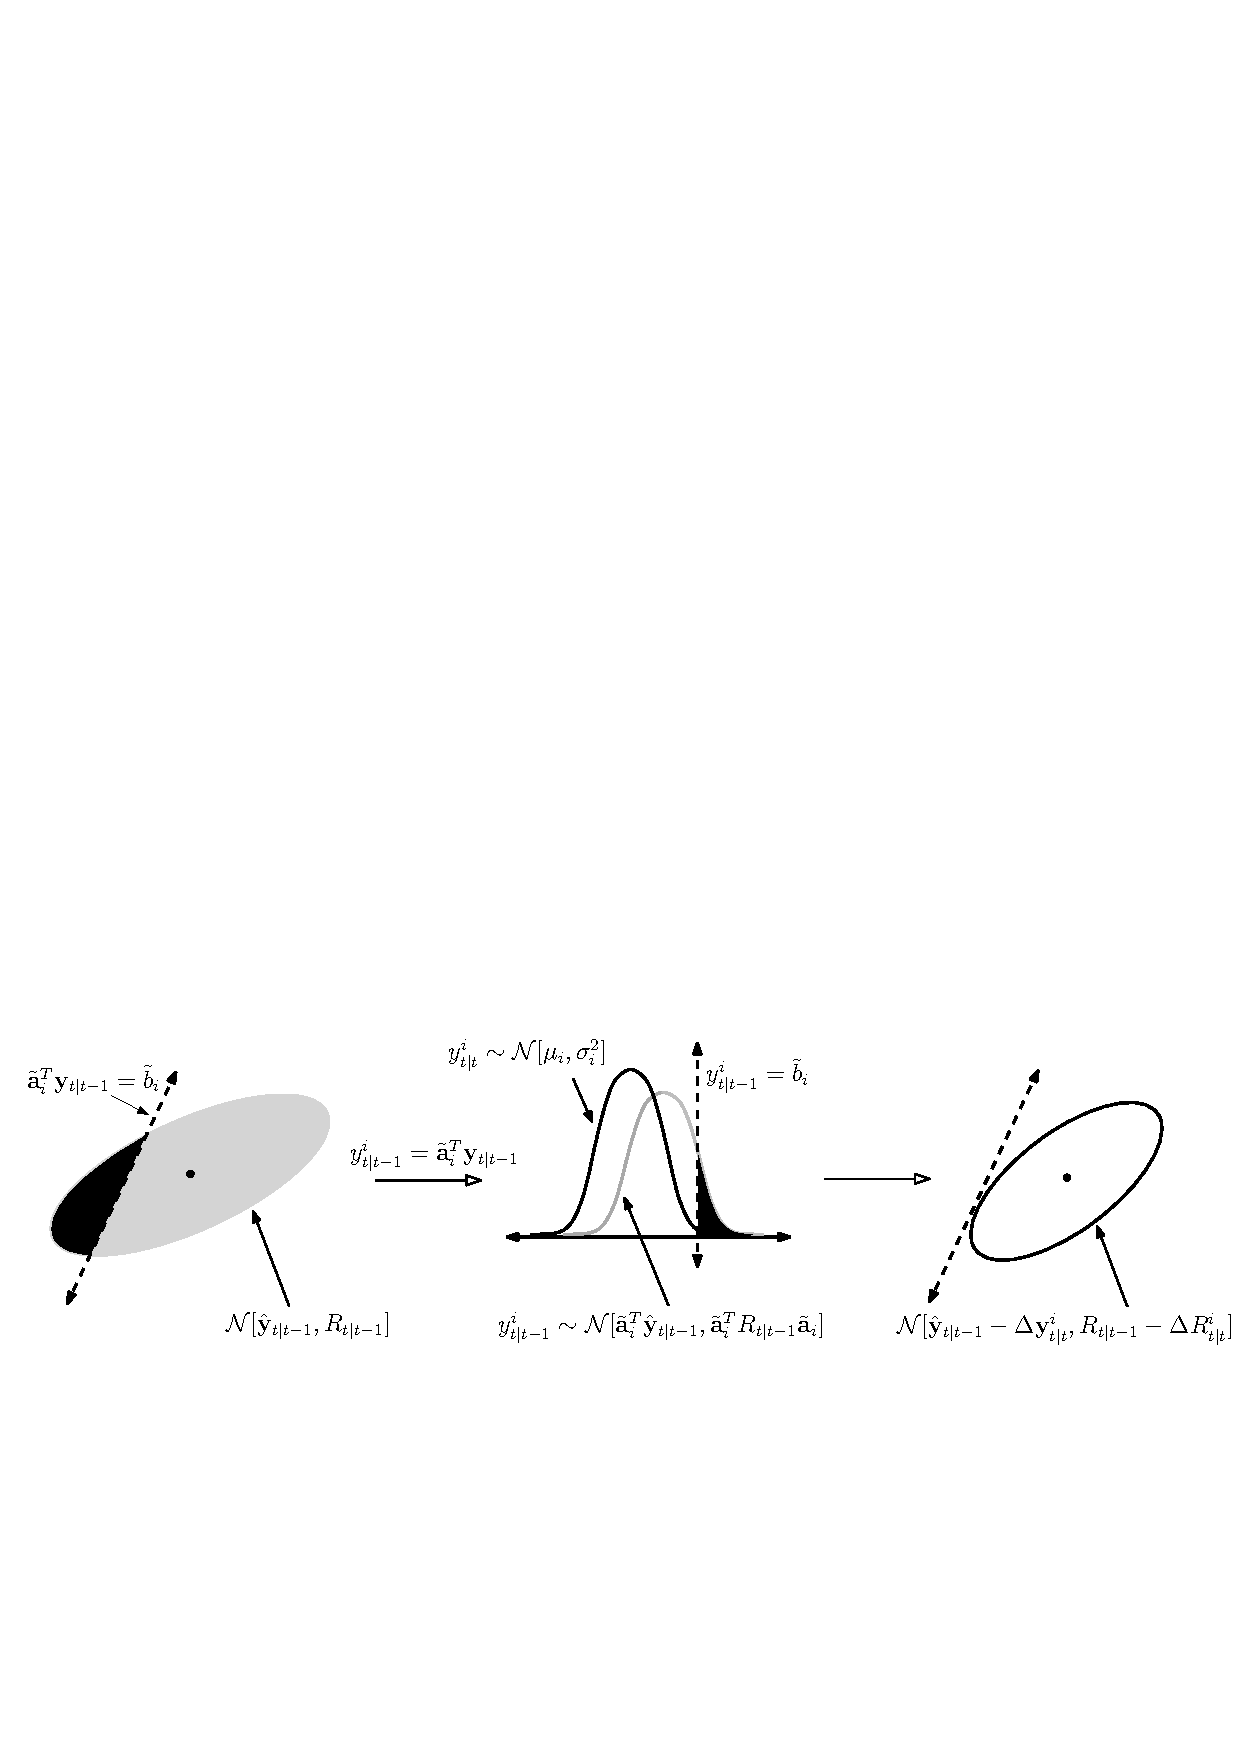
\includegraphics[width=480pt,clip]{figures/truncation2.pdf}
\vspace{-5pt}
\caption{The joint conditional distribution $\mathbf{y}_{t|t-1} \sim \mathcal{N}[\hat{\mathbf{y}}_{t|t-1}, R_{t|t-1}]$ (left), is truncated with respect to the $i^\textrm{th}$ constraint $\tilde{\mathbf{a}}_i^T \mathbf{y}_{t|t-1} \leq \tilde{b}_i$, in $\mathbb{R}^{2n_x}$. Applying an affine transformation, $y^i_{t|t-1} = \tilde{\mathbf{a}}_i^T\mathbf{y}_{t|t-1}$, transforms the distribution to a 1D Gaussian $y_{t|t-1}^i \sim \mathcal{N}[\tilde{\mathbf{a}}_i^T\hat{\mathbf{y}}_{t|t-1}, \tilde{\mathbf{a}}_i^T R_{t|t-1} \tilde{\mathbf{a}}_i]$ (middle). The area under the 1D Gaussian that lies beyond the constraint $y^i_{t|t-1} = \tilde{b}_i$ (shaded in black), gives the probability of collision of the robot with the $i^\textrm{th}$ constraint. We estimate the truncated distribution in $\mathbb{R}^{2n_x}$ by conditioning on the truncated 1D Gaussian $y_{t|t}^i \sim \mathcal{N}[\mu_i, \sigma_i^2]$ (right). The mean $(\hat{\mathbf{y}}_{t|t-1} - \Delta \mathbf{y}_{t|t}^i)$, and variance $(R_{t|t-1} - \Delta R_{t|t}^i)$, of the distribution $\mathbf{y}_{t|t}$ after truncation are obtained by accumulating the effects of truncation with respect to all constraints (order independent).}
\label{fig:truncation}
\vspace*{-10pt}
\end{figure*}

At each stage $t$ of the plan, we approximate the distribution of the feasible robot states with a truncated Gaussian distribution \cite{Book:Johnson94}. For the sake of brevity, we assume that the feasible region containing the state at each stage $t$ is convex and is described by the conjunction of $k$ linear inequality constraints as $\bigcap_{i = 0}^{k} \mathbf{a}_i\mathbf{x}_t \leq b_i$. We later extend this analysis in Sec. \ref{sec:cvxfn} to non-convex regions by constructing a locally convex feasible region around the robot state.

Since the true state deviation and its estimate are correlated (Eqn. \ref{eq:jointevolve}), it is important to truncate the joint conditional distribution $\mathcal{N}[\hat{\mathbf{y}}_{t|t-1}, R_{t|t-1}]$ in $\mathbb{R}^{2n_x}$, with respect to the $k$ constraints. The $i^{\textrm{th}}$ linear constraint is then represented in $\mathbb{R}^{2n_x}$ as $\tilde{\mathbf{a}}_i^T \mathbf{y}_{t|t-1} \leq \tilde{b}_i$, where $\tilde{\mathbf{a}}_i = \left[\begin{smallmatrix} \mathbf{a}_i \\ \mathbf{0} \end{smallmatrix} \right]$, and $\tilde{b}_i = (b_i - \mathbf{a}_i^T\mathbf{x}^{\star}_t)$.

We truncate the joint conditional distribution with respect to each constraint in a sequential manner and then accumulate the effect of truncation over all the constraints. In contrast to prior methods that use truncated distributions \cite{Book:Simon06, Toussaint09_NIPS}, we propose a novel truncation method that does not depend on the order in which the constraints are processed. Given the $i^{\textrm{th}}$ constraint $\tilde{\mathbf{a}}_i^T \mathbf{y}_{t|t-1} \leq \tilde{b}_i$, we apply an affine transformation $y^i_{t|t-1} = \tilde{\mathbf{a}}_i^T\mathbf{y}_{t|t-1}$ to transform the conditional distribution $\mathcal{N}[\hat{\mathbf{y}}_{t|t-1}, R_{t|t-1}]$, to a 1D Gaussian $\mathcal{N}[\tilde{\mathbf{a}}_i^T\hat{\mathbf{y}}_{t|t-1}, \tilde{\mathbf{a}}_i^T R_{t|t-1} \tilde{\mathbf{a}}_i]$ along an axis normal to the constraint (as shown in Fig. \ref{fig:truncation}). The problem now simplifies to truncating the 1D Gaussian distribution at a specified upper bound given by $y^i_{t|t-1} = \tilde{b}_i$, which is well-known from standard statistical literature \cite{Book:Johnson94}. The mean, $\mu_i$, and variance, $\sigma^2_i$, of the truncated 1D Gaussian $y_{t|t}^i$ is given by:
\begin{align}
\mu_i &= \tilde{\mathbf{a}}_i^T\hat{\mathbf{y}}_{t|t-1} + \lambda(\alpha_i)\sqrt{\tilde{\mathbf{a}}_i^T R_{t|t-1} \tilde{\mathbf{a}}_i}, \label{eq:1DtruncMu}\\
\sigma^2_i &= \tilde{\mathbf{a}}_i^T R_{t|t-1} \tilde{\mathbf{a}}_i (1 - \lambda(\alpha_i)^2 + \alpha_i \lambda(\alpha_i)) \label{eq:1DtruncSigma},
\end{align}
where
\begin{equation} \label{eq:alpha}
\alpha_i = \frac{(\tilde{b}_i - \tilde{\mathbf{a}}_i^T\hat{\mathbf{y}}_{t|t-1})}{\sqrt{\tilde{\mathbf{a}}_i^T R_{t|t-1} \tilde{\mathbf{a}}_i}}, ~~~ \lambda(\alpha_i) = \frac{\textrm{pdf}(\alpha_i)}{\textrm{cdf}(\alpha_i)}.
\end{equation}
$\lambda(\alpha_i)$ is the ratio of the standard Gaussian (mean $0$ and variance $1$) probability distribution function and the standard Gaussian cumulative distribution function evaluated at $\alpha_i$. Note that $(1 - \textrm{cdf}(\alpha_i))$ is the area under the Gaussian that lies beyond the constraint (shaded in black in Fig. \ref{fig:truncation}), and is the probability that the robot lies in the infeasible region corresponding to the $i^\textrm{th}$ constraint.
%$\alpha_i = \frac{(\tilde{b}_i - \tilde{\mathbf{a}}_i^T\hat{\mathbf{y}}_t)}{\sqrt{\tilde{\mathbf{a}}_i^T R_t \tilde{\mathbf{a}}_i}}$, and $\lambda(\alpha_i) = \frac{\textrm{pdf}(\alpha_i)}{\textrm{cdf}(\alpha_i)}$, is the ratio of the Gaussian probability distribution function and the Gaussian cumulative distribution function evaluated at $y'_t = \alpha_i$. Note that $(1 - \textrm{cdf}(\alpha_i))$ is the area under the Gaussian (shaded in black in Fig. \ref{fig:truncation}) that lies beyond the truncation limit $\tilde{b}_i$, and is the probability that the robot lies in the infeasible region corresponding to the $i^\textrm{th}$ constraint.

The mean and variance of the truncated distribution $\mathbf{y}_{t|t}$ can be found by conditioning the joint distribution $(\mathbf{y}_{t|t-1},y^i_{t|t-1})$, on the truncated 1D distribution $y^i_{t|t}$: $\mathbf{y}_{t|t} = (\mathbf{y}_{t|t-1}|y^i_{t|t-1}=y^i_{t|t})$ (see appendix). The shift in the mean due to truncation with respect to the $i^\textrm{th}$ constraint is given by:
\begin{equation} \label{eq:truncmean}
\Delta \mathbf{y}^i_t = \frac{R_{t|t-1}\tilde{\mathbf{a}}_i}{\tilde{\mathbf{a}}_i^T R_{t|t-1} \tilde{\mathbf{a}}_i}(\tilde{\mathbf{a}}_i^T\hat{\mathbf{y}}_{t|t-1} - \mu_i),
\end{equation}
and the shift in variance is given by:
\begin{equation} \label{eq:truncvar}
\Delta R^i_t = \frac{R_{t|t-1}\tilde{\mathbf{a}}_i}{\tilde{\mathbf{a}}_i^T R_{t|t-1} \tilde{\mathbf{a}}_i}(\tilde{\mathbf{a}}_i^TR_{t|t-1}\tilde{\mathbf{a}}_i - \sigma_i^2)\frac{\tilde{\mathbf{a}}_i^TR_{t|t-1}}{\tilde{\mathbf{a}}_i^T R_{t|t-1} \tilde{\mathbf{a}}_i}.
\end{equation}

Given $k$ constraints, the cumulative shift in the mean due to truncation is then given by $\Delta \mathbf{y}_{t|t} = \sum_{i = 0}^{k} \Delta \mathbf{y}^i_{t|t}$, and the cumulative shift in variance is given by $\Delta R_{t|t} = \sum_{i = 0}^{k} \Delta R^i_{t|t}$. The mean and variance of the truncated conditional distributions are then propagated recursively using Eqs.\ (\ref{eq:newjointmean}) and (\ref{eq:newjointvar}).

The truncation method described here is general enough to handle constraints on the entire robot state. Examples of such constraints include spatial constraints imposed on the position of the robot by obstacles in the environment or limits imposed on other state variables such as the velocity and acceleration of the robot. Our method had the added advantage that it is independent of the order in which constraints are processed, which eliminates convergence issues related to handling state constraints in several optimization \cite{Platt10_RSS, Erez10_UAI, vandenBerg11_ISRR} and inference based \cite{Toussaint09_ICML} planning methods.

\subsection{Estimating the Probability of Collision} \label{sec:estprob}

We use the truncated conditional distributions to estimate the overall probability of collision of the given plan, based on the conditional probabilities of collisions at each stage along the plan. Given the joint conditional distribution at stage $t$, $\mathcal{N}[\hat{\mathbf{y}}_{t|t-1}, R_{t|t-1}]$, and the set of $k$ linear constraints that define the locally convex region of free space containing the robot, we compute a lower bound for the probability of the robot being collision free using Boole's inequality, as \cite{Vitus11_ICRA}:
\begin{align} \label{eq:probboole}
p(\mathbf{x}_{t|t-1} \in \mathcal{X}_{F}) &\geq 1 - p\bigl(\bigvee_{i = 0}^{k} \; \tilde{\mathbf{a}}_i^T \hat{\mathbf{y}}_{t|t-1} > \tilde{b}_i \bigr)\nonumber\\
&\geq 1 - \sum_{i = 0}^{k} (1 - \textrm{cdf} (\alpha_i)).
\end{align}

The overall probability that the robot does not collide with any obstacle for the duration $\ell$ of the plan, is given by:
\begin{equation} \label{eq:probsuccess}
p(\bigwedge_{t = 0}^{\ell} \mathbf{x}_t \in \mathcal{X}_{F}) = \prod_{t = 0}^{\ell} p(\mathbf{x}_{t|t-1} \in \mathcal{X}_{F}),
\end{equation}
and the overall probability of collision is provided by the complement $(1 - p(\bigwedge_{t = 0}^{\ell} \mathbf{x}_t \in \mathcal{X}_{F}))$. 